% ═══════════════════════════════════════════════════════════════════════════
\section{Esperimenti e Visualizzazione Interattiva}\label{sec:esperimenti}
% ═══════════════════════════════════════════════════════════════════════════

In questo capitolo descriviamo l'ambiente sperimentale utilizzato per
validare gli algoritmi del Capitolo~\ref{sec:algoritmi}, l'architettura
software dell'applicazione web interattiva e i risultati numerici ottenuti,
confrontando il metodo del gradiente a campione dinamico con SGD e batch
gradient descent, e Newton-CG con il gradiente dinamico. I listati Python
completi sono riportati nell'Appendice~\ref{app:listati}.

\subsection{Setup Sperimentale}\label{sec:setup}

Gli esperimenti sono condotti in un ambiente di \emph{simulazione}: le
funzioni obiettivo e i dataset sono generati sinteticamente, seguendo la
costruzione del ``dataset centrato'' descritta nella
Sezione~\ref{sec:architettura}. In questo modo si può controllare esattamente
la soluzione $w^*$ e la struttura del problema, e misurare l'errore finale
$\|w_k - w^*\|$ senza ambiguità.

Le funzioni test utilizzate sono le seguenti.

\begin{itemize}
  \item \textbf{Quadratica (regressione lineare).} La perdita è
  $J(w) = \frac{1}{2N}\sum_{i=1}^{N}(x_i^T w - y_i)^2$, con $N = 1000$ esempi,
  $m = 10$ variabili, dati $x_i$ generati da una gaussiana standard e
  $y_i = x_i^T w_{\mathrm{true}} + \varepsilon_i$ con rumore gaussiano.
  Il numero di condizionamento misurato è $\kappa \approx 1.4$.
  \item \textbf{Quadratica mal condizionata.} Come sopra, ma con feature
  correlate tra loro, in modo da ottenere $\kappa \approx 107$. Questo
  problema è rappresentativo dei dataset reali, dove le caratteristiche sono
  spesso ridondanti.
  \item \textbf{Rosenbrock.} La funzione di Rosenbrock
  $J(w) = \sum_{j=1}^{m-1}\bigl[100(w_{j+1}-w_j^2)^2 + (1-w_j)^2\bigr]$,
  con minimo $w^* = (1,\dots,1)$, è usata come esempio di funzione non
  quadratica con valle stretta e curvatura fortemente variabile. Come
  discusso nella Sezione~\ref{sec:risultati}, i metodi del primo ordine
  falliscono su questo problema, mentre Newton-CG converte rapidamente.
\end{itemize}

Per ogni problema test, la dimensione del dataset è $N = 1000$ e la
dimensionalità è $m = 10$. Il punto iniziale è $w_0 = (2,\dots,2)$ e la
tolleranza per il criterio di arresto $\|\nabla J(w_k)\|_2 < 10^{-6}$. Per il
metodo dinamico sono stati testati i valori $\theta \in \{0.1, 0.5, 0.9\}$
della tolleranza nella Condizione di Controllo della Varianza, con dimensione
iniziale del batch $n_0 = 16$; per Newton-CG il rapporto di sottocampionamento
dell'Hessiana è $R = 0.1$. Il confronto include il gradiente stocastico (SGD)
con batch unitario e passo $1/(\lambda k)$, e il gradiente batch completo
con passo $1/L$.

Tutti gli esperimenti sono stati eseguiti su un computer portatile con
processore Apple Silicon (8 core) e 16~GB di RAM, in ambiente macOS, con
Python~3.14, NumPy~2.4 e Matplotlib~3.11. Non è richiesto alcun acceleratore
GPU. I tempi riportati sono tempi di esecuzione \emph{medi} su una singola
esecuzione per ogni configurazione.

\subsection{Architettura Software}\label{sec:architettura}

Per rendere concreti i concetti teorici esposti nel
Capitolo~\ref{sec:algoritmi}, è stata realizzata un'\textbf{applicazione web
interattiva} che implementa i tre algoritmi in un ambiente visivo e
modificabile dall'utente. Il codice sorgente è disponibile al seguente
repository GitHub:
\begin{center}
  \url{https://github.com/alessandrolocurcio/selezione-dinamica-batch}
\end{center}
%(NOTA: sostituire con l'URL effettivo del repository o del notebook Colab.)

L'applicazione esegue il codice Python (funzione obiettivo, gradiente,
algoritmo) \emph{direttamente nel browser} tramite il runtime Python
Pyodide, consentendo all'utente di modificare loss e algoritmo e vedere
immediatamente il risultato. La visualizzazione delle superfici e dei
percorsi di ottimizzazione è affidata a Plotly (libreria JavaScript).
L'interfaccia permette di:

\begin{itemize}
  \item selezionare o scrivere una funzione obiettivo $J(w)$ con gradiente
  $\nabla J(w)$ e Hessiana $\nabla^2 J(w)$, scegliendo tra preset predefiniti
  o codice personalizzato;
  \item scegliere tra i tre algoritmi discussi (gradiente dinamico,
  Newton-CG con campionamento dinamico, Newton-CG con regolarizzazione
  $L_1$), il cui codice Python è visibile e modificabile;
  \item variare i parametri dell'algoritmo in tempo reale;
  \item visualizzare il percorso di ottimizzazione sulla superficie di
  $J(w)$ (in 3D per funzioni 2D, in 2D per funzioni 1D), con possibilità di
  scorrere le iterazioni, avviare una riproduzione automatica e ruotare la
  visualizzazione;
  \item monitorare metriche in tempo reale (valore di $J(w_k)$, norma del
  gradiente, dimensione del batch);
  \item eseguire un'analisi di convergenza che mostra l'errore e $J(w_k)$
  per ogni iterazione.
\end{itemize}


\paragraph{Costruzione del dataset sintetico centrato.}
Nel codice dell'applicazione, la superficie plottata è la funzione obiettivo
teorica $J(w)$, definita dall'utente nel preset della loss. Questa è la
funzione che si vorrebbe minimizzare: viene usata per disegnare il grafico,
per calcolare i valori del percorso e per mostrare le metriche come $J(w_k)$
e $\|\nabla J(w_k)\|$. L'algoritmo però non minimizza direttamente $J(w)$,
ma utilizza un dataset sintetico di $N$ funzioni di perdita individuali
$\ell(w; i)$, con $i = 1,\dots,N$, costruito a partire da $J(w)$ perturbando
i suoi coefficienti; ogni funzione $\ell(w; i)$ rappresenta il contributo del
singolo esempio $i$. A ogni iterazione l'algoritmo seleziona un batch
$\mathcal{S}_k$ di dimensione $n_k$ e calcola il gradiente del batch come
$g_k = \frac{1}{n_k}\sum_{i \in \mathcal{S}_k}\nabla \ell(w_k; i)$; la line
search di Armijo usa la loss del batch
$J_{\mathcal{S}_k}(w) = \frac{1}{n_k}\sum_{i \in \mathcal{S}_k}\ell(w; i)$.
La media su tutti gli $N$ dati è
$\hat J_N(w) = \frac{1}{N}\sum_{i=1}^N \ell(w; i)$.

Il dataset è costruito in modo che le medie campionarie dei coefficienti
delle perturbazioni coincidano \emph{esattamente} con i coefficienti di
$J(w)$; pertanto $\hat J_N(w) = J(w)$ per ogni $w$ e
$\nabla \hat J_N(w) = \nabla J(w)$ per ogni $w$, indipendentemente da $N$.
Questa proprietà è ottenuta sottraendo a ogni perturbazione la propria media
campionaria. Quindi $J(w)$ è la funzione plottata, mentre l'algoritmo
minimizza $\hat J_N(w)$ (o sue approssimazioni su batch). Nel codice
$\hat J_N(w)$ coincide esattamente con $J(w)$ per ogni $N$, a differenza di
un problema reale dove la coincidenza si ha solo nel limite $N \to \infty$.
In sintesi, la loss teorica $J(w)$ è usata per il plot e le metriche, la loss
campionaria totale $\hat J_N(w)$ per la condizione di arresto, la loss del
batch $J_{\mathcal{S}_k}(w)$ per la line search, e il gradiente del batch
$g_k$ per l'aggiornamento dei pesi.

L'implementazione segue la struttura algoritmica del
Capitolo~\ref{sec:algoritmi}, con due estensioni rispetto alla formulazione
originale~\cite{byrd2012}: la CCV estesa al subgradiente per $L_1$ (nel
paper il sample size per il caso $L_1$ è assunto fisso, e gli autori
lasciano l'estensione al caso dinamico come lavoro futuro) e il dataset
sintetico centrato descritto sopra. Per il resto, l'implementazione è fedele
al paper: l'Hessiana nel Newton-CG è calcolata su un sottocampione di
dimensione $|\mathcal{H}_k| = R \cdot |\mathcal{S}_k|$; il CG per il caso
$L_1$ usa la tolleranza fissa $\eta$ della \eqref{eq:cg_l1}; la line search
di Wolfe è quella degli algoritmi pratici del paper, mentre i passi fissi
compaiono solo nell'analisi teorica di complessità.

\subsection{Risultati Numerici}\label{sec:risultati}

Presentiamo i risultati numerici ottenuti nel setup descritto nella
Sezione~\ref{sec:setup}. La Tabella~\ref{tab:6_1} confronta il metodo del
gradiente a campione dinamico (Dynamic GD) con SGD e batch gradient descent
(Batch GD) sui due problemi quadratici. La Tabella~\ref{tab:6_2} confronta
Newton-CG con Dynamic GD.

\begin{table}[h]
\centering
\small
\renewcommand{\arraystretch}{1.3}
\begin{tabular}{l l r r r r}
\toprule
\textbf{Metodo} & \textbf{Parametro} & \textbf{Iterazioni} &
\textbf{Tempo (s)} & \textbf{Errore} & \textbf{Max batch} \\
\midrule
% Righe della Tabella 6.1 (columns: Metodo & Parametro & Iterazioni & Tempo & Errore & Max batch)
\multicolumn{6}{l}{\textbf{Quadratica}\ ($\kappa \approx 1.4$)} \\ \hline
  Dynamic GD & $\theta=0.1$ & 14 & 0.03 & $6.47\times10^{-7}$ & 1000 \\
  Dynamic GD & $\theta=0.5$ & 18 & 0.02 & $6.34\times10^{-7}$ & 1000 \\
  Dynamic GD & $\theta=0.9$ & 45 & 0.03 & $1.13\times10^{-6}$ & 1000 \\
  SGD & $n=1$ & 300 & $<0.01$ & $4.45\times10^{-1}$ & 1 \\
  Batch GD & $n=N$ & 14 & $<0.01$ & $1.46\times10^{-7}$ & 1000 \\
\hline
\multicolumn{6}{l}{\textbf{Quadratica mal condizionata}\ ($\kappa \approx 107$)} \\ \hline
  Dynamic GD & $\theta=0.1$ & 300 & 12.82 & $2.66\times10^{0}$ & 1000 \\
  Dynamic GD & $\theta=0.5$ & 300 & 7.33 & $3.09\times10^{-1}$ & 1000 \\
  Dynamic GD & $\theta=0.9$ & 300 & 3.21 & $2.03\times10^{-1}$ & 992 \\
  SGD & $n=1$ & 300 & $<0.01$ & $4.11\times10^{-1}$ & 1 \\
  Batch GD & $n=N$ & 300 & $<0.01$ & $4.99\times10^{-2}$ & 1000 \\

\bottomrule
\end{tabular}
\caption{Confronto tra Dynamic GD, SGD e Batch GD sui problemi quadratici.
Per ogni configurazione sono riportate le iterazioni totali, il tempo di
esecuzione, l'errore finale $\|w_k - w^*\|$ e la dimensione massima del batch
raggiunta dal metodo dinamico. SGD non raggiunge la tolleranza
$\|\nabla J\| < 10^{-6}$ entro il budget di 300 iterazioni.}
\label{tab:6_1}
\end{table}

\begin{table}[h]
\centering
\small
\renewcommand{\arraystretch}{1.3}
\begin{tabular}{l l r r r r}
\toprule
\textbf{Metodo} & \textbf{Parametro} & \textbf{Iter.\ est.} &
\textbf{Iter.\ medie CG} & \textbf{Tempo (s)} & \textbf{Errore} \\
\midrule
% Righe della Tabella 6.2 (columns: Metodo & Parametro & Iter. est. & Iter. medie CG & Tempo & Errore)
\multicolumn{6}{l}{\textbf{Quadratica}\ ($\kappa \approx 1.4$)} \\ \hline
  Newton-CG & $R=0.1$ & 18 & 1.1 & 0.03 & $5.53\times10^{-7}$ \\
  Dynamic GD & $\theta=0.5$ & 18 & --- & 0.02 & $6.34\times10^{-7}$ \\
\hline
\multicolumn{6}{l}{\textbf{Quadratica mal condizionata}\ ($\kappa \approx 107$)} \\ \hline
  Newton-CG & $R=0.1$ & 66 & 1.9 & 0.24 & $1.95\times10^{-5}$ \\
  Dynamic GD & $\theta=0.5$ & 300 & --- & 7.33 & $3.09\times10^{-1}$ \\

\bottomrule
\end{tabular}
\caption{Confronto tra Newton-CG e gradiente a campione dinamico. Sono
riportate le iterazioni esterne, le iterazioni medie del gradiente coniugato
interno e l'errore finale. Newton-CG riduce drasticamente il numero di
iterazioni sul problema mal condizionato.}
\label{tab:6_2}
\end{table}



Le figure seguenti illustrano il comportamento qualitativo del metodo. La
Figura~\ref{fig:convergenza} mostra la convergenza del gradiente a campione
dinamico sul problema quadratico ben condizionato per i tre valori di
$\theta$: come previsto dalla teoria, l'errore $J(w_k) - J(w_*)$ decresce
linearmente (scala logaritmica), con una pendenza che dipende da $\theta$.
La Figura~\ref{fig:batch} mostra l'evoluzione della dimensione del batch
$n_k$: il batch cresce a scalini quando la CCV viene violata, e rimane invece
costante nel caso di batch fisso. La Figura~\ref{fig:bar} confronta il costo
totale in valutazioni di gradienti individuali entro un budget di 300
iterazioni: Dynamic GD usa molte meno valutazioni di Batch GD (che valuta
l'intero dataset a ogni iterazione) e, a differenza di SGD, raggiunge la
precisione richiesta.

\begin{figure}[h]
\centering
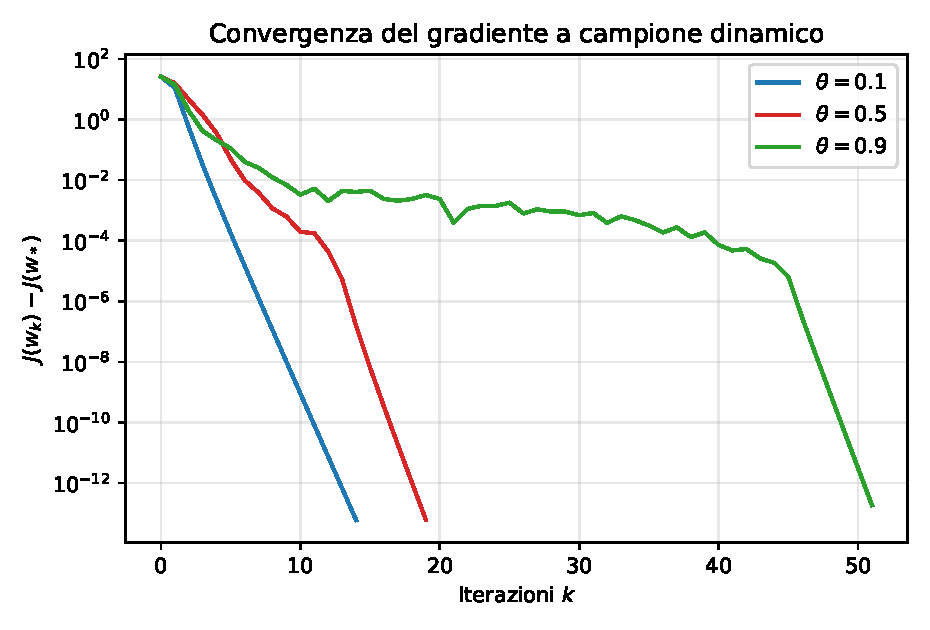
\includegraphics[width=0.78\textwidth]{figure/convergenza.pdf}
\caption{Convergenza $J(w_k) - J(w_*)$ in scala logaritmica del metodo del
gradiente a campione dinamico sul problema quadratico ($\kappa \approx 1.4$)
per $\theta \in \{0.1, 0.5, 0.9\}$.}
\label{fig:convergenza}
\end{figure}

\begin{figure}[h]
\centering
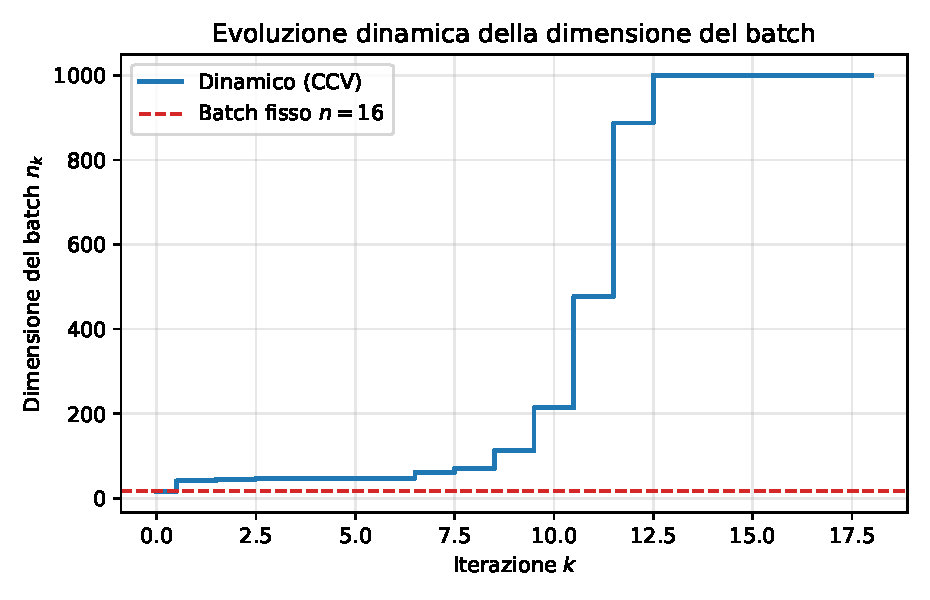
\includegraphics[width=0.78\textwidth]{figure/batch_size.pdf}
\caption{Evoluzione della dimensione del batch $n_k$ con la strategia
dinamica (CCV) rispetto a un batch fisso. Il batch cresce automaticamente
quando ci si avvicina al minimo.}
\label{fig:batch}
\end{figure}

\begin{figure}[h]
\centering
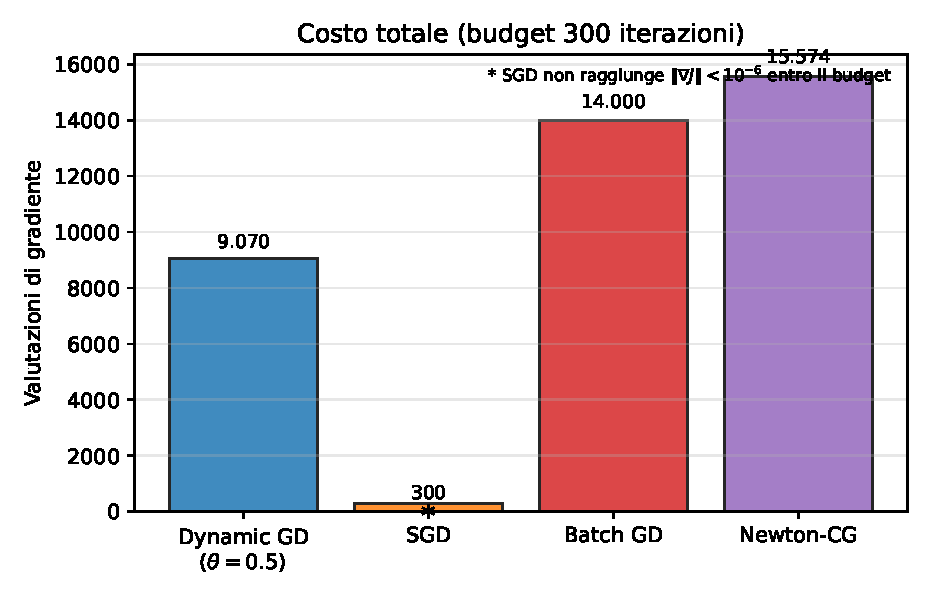
\includegraphics[width=0.78\textwidth]{figure/bar_comparison.pdf}
\caption{Numero totale di valutazioni di gradienti individuali entro un
budget di 300 iterazioni sul problema quadratico ben condizionato. SGD non
raggiunge la tolleranza $\|\nabla J\| < 10^{-6}$ entro il budget.}
\label{fig:bar}
\end{figure}

Dalla Tabella~\ref{tab:6_1} emergono tre osservazioni. In primo luogo, sul
problema ben condizionato il metodo dinamico converge in poche iterazioni
(14--45) con un errore dell'ordine di $10^{-6}$-$10^{-7}$, a fronte di un
costo per iterazione che cresce progressivamente: la CCV aumenta il batch
fino alla dimensione massima $N$ proprio quando il gradiente si avvicina a
zero, concentrando la risorsa computazionale dove serve precisione. In
secondo luogo, SGD con passo $1/(\lambda k)$ non riesce a scendere al di
sotto di un errore dell'ordine di $10^{-1}$: il rumore stocastico limita la
precisione, come previsto dalla teoria. In terzo luogo, sul problema mal
condizionato tutti i metodi del primo ordine degradano sensibilmente:
Dynamic GD e Batch GD richiedono le 300 iterazioni del budget senza
raggiungere la tolleranza, a causa del numero di condizionamento elevato.

La Tabella~\ref{tab:6_2} mostra il vantaggio dell'informazione di curvatura:
sul problema mal condizionato Newton-CG converge in 66 iterazioni esterne
(con in media meno di 2 iterazioni del CG interno per iterazione) e raggiunge
un errore di $1.95\times10^{-5}$, mentre Dynamic GD non converge nel budget
disponibile. Il criterio di arresto adattivo del CG evita iterazioni interne
inutili: le iterazioni medie del CG sono molto basse, poiché il CG viene
fermato quando il residuo è confrontabile con l'errore di approssimazione
dell'Hessiana.

Infine, il problema di Rosenbrock (non quadratico, con valle stretta)
conferma qualitativamente le conclusioni: i metodi del primo ordine, incluso
Dynamic GD con la strategia dinamica, restano intrappolati nella valle e non
raggiungono il minimo in 300 iterazioni, mentre Newton-CG sfrutta la
curvatura dell'Hessiana (esatta, in questo caso) e scende rapidamente lungo
la valle. Questi risultati motivano l'uso di metodi di secondo ordine per
problemi difficili, in accordo con l'analisi teorica del
Capitolo~\ref{sec:algoritmi}.

\subsection{Visualizzazione Interattiva}\label{sec:visualizzazione}

L'applicazione web descritta nella Sezione~\ref{sec:architettura} consente
di osservare direttamente i concetti teorici discussi in questa tesi.
L'utente può:

\begin{itemize}
  \item \textbf{sperimentare l'effetto di $\theta$}: selezionando un valore
  piccolo di $\theta$, la CCV diventa stringente e il batch cresce presto; con
  $\theta$ grande, il batch resta piccolo più a lungo e l'algoritmo procede
  più rapidamente, ma con un errore finale più alto;
  \item \textbf{osservare la dinamica del batch}: il grafico della dimensione
  del batch in funzione dell'iterazione mostra i ``gradini'' di crescita,
  che si verificano esattamente quando la varianza stimata supera la soglia;
  \item \textbf{confrontare i tre algoritmi} sulla stessa funzione obiettivo,
  variando in tempo reale i parametri (batch iniziale, rapporto $R$, passo,
  regolarizzazione $\nu$), e visualizzando i percorsi sovrapposti sulla
  superficie di $J(w)$;
  \item \textbf{studiare la convergenza}: la tabella delle iterazioni riporta
  $J(w_k)$ e l'errore, permettendo di verificare empiricamente il tasso di
  convergenza lineare del metodo dinamico;
  \item \textbf{modificare il codice}: il codice Python di ogni algoritmo è
  visibile e modificabile nel browser, consentendo di introdurre varianti e di
  verificarne l'effetto senza installare nulla.
\end{itemize}

Il codice completo degli algoritmi eseguiti nell'applicazione è riportato
nell'Appendice~\ref{app:listati}; le istruzioni per l'esecuzione e per
l'avvio dell'applicazione sono nell'Appendice~\ref{app:istruzioni}.

